% ============================================================
% Provisional Results and Discussion draft for EAAI
% Generated only from the four phase-1 CSV exports in source_data/.
% No missing result is interpolated. Conditional rankings must be updated
% when the remaining benchmark and robustness runs are available.
% ============================================================

\section{Results and Discussion}
\label{sec:results_discussion}

\subsection{Phase-1 Evidence Scope and Reporting Strategy}
\label{subsec:phase1_scope}

This section reports the first completed experimental block and is intentionally
restricted to the evidence contained in the current exports. The benchmark file
contains 52 unique model--dataset evaluations over CIF, M3, M4, and Tourism.
All 16 candidate models are available for CIF and M3, whereas M4 and Tourism
currently contain 10 models and do not yet include CNN, LSTM, DLinear, NLinear,
Chronos-Bolt-Small, or TimesFM-2.5-200M. Consequently, the ranks reported for
M4 and Tourism are conditional on the completed runs and are not final
cross-model rankings.

The error distributions are strongly right-skewed. In the data-efficiency
export, the ratio between mean and median MAPE reaches several orders of
magnitude for some cells, consistent with the instability of percentage errors
when individual targets approach zero. Median MAPE is therefore used as the
primary descriptive statistic, with the interquartile range (IQR), MASE, and
empirical coverage probability (ECP) used as complementary evidence. This
choice prevents a small number of pathological percentage errors from
dominating the cross-series interpretation, but it does not remove the known
limitations of MAPE.

The anonymized Industrial Construction-Materials Demand (ICMD) application
remains the primary engineering use case. Its source contains 61,395
transactional records, 47 variables, 555 product references, and 62 monthly
periods between January 2020 and February 2025. The evaluated product series
contains 48 monthly observations, with the final 10 months reserved for test.
The current phase-1 exports do not contain the finalized ICMD benchmark rows;
therefore, no ICMD accuracy or shock-robustness claim is made in this draft.
Those results will be inserted without altering the analyses reported below.

\subsection{Overall Benchmark Performance}
\label{subsec:benchmark_results}

Table~\ref{tab:phase1_benchmark} and
Fig.~\ref{fig:benchmark_mape_phase1} show that the relative performance of the
S3 family is dataset dependent rather than uniformly dominant. This result is
important because the proposed architectures are intended as controlled
residual adapters, not as universal replacements for every statistical
forecaster.

\begin{table*}[t]
\centering
\caption{Phase-1 benchmark summary based on median MAPE. Only completed model--dataset evaluations are ranked.}
\label{tab:phase1_benchmark}
\footnotesize
\setlength{\tabcolsep}{4pt}
\begin{tabular}{lrrrrlrlr}
\toprule
& \multicolumn{2}{c}{S3-FastSketch} & \multicolumn{2}{c}{S3-Forecaster}
& \multicolumn{2}{c}{Overall best} & \multicolumn{2}{c}{Best non-S3} \\
\cmidrule(lr){2-3}\cmidrule(lr){4-5}\cmidrule(lr){6-7}\cmidrule(lr){8-9}
Dataset & Rank & MAPE (\%) & Rank & MAPE (\%) & Model & MAPE (\%) & Model & MAPE (\%) \\
\midrule
CIF & 1 & 5.00 & 2 & 5.13 & S3-FastSketch & 5.00 & ETS & 5.19 \\
M3 & 11 & 8.80 & 6 & 7.04 & ETS & 5.44 & ETS & 5.44 \\
M4 & 7 & 3.97 & 8 & 4.05 & GPR & 2.97 & GPR & 2.97 \\
Tourism & 1 & 16.64 & 4 & 18.09 & S3-FastSketch & 16.64 & ETS & 17.32 \\
\bottomrule
\end{tabular}
\begin{minipage}{0.98\textwidth}
\footnotesize\emph{Note:} Ranks are conditional on the available phase-1 results and must not be interpreted as final rankings until the missing model--dataset runs are completed.
\end{minipage}
\end{table*}


\begin{figure*}[t]
    \centering
    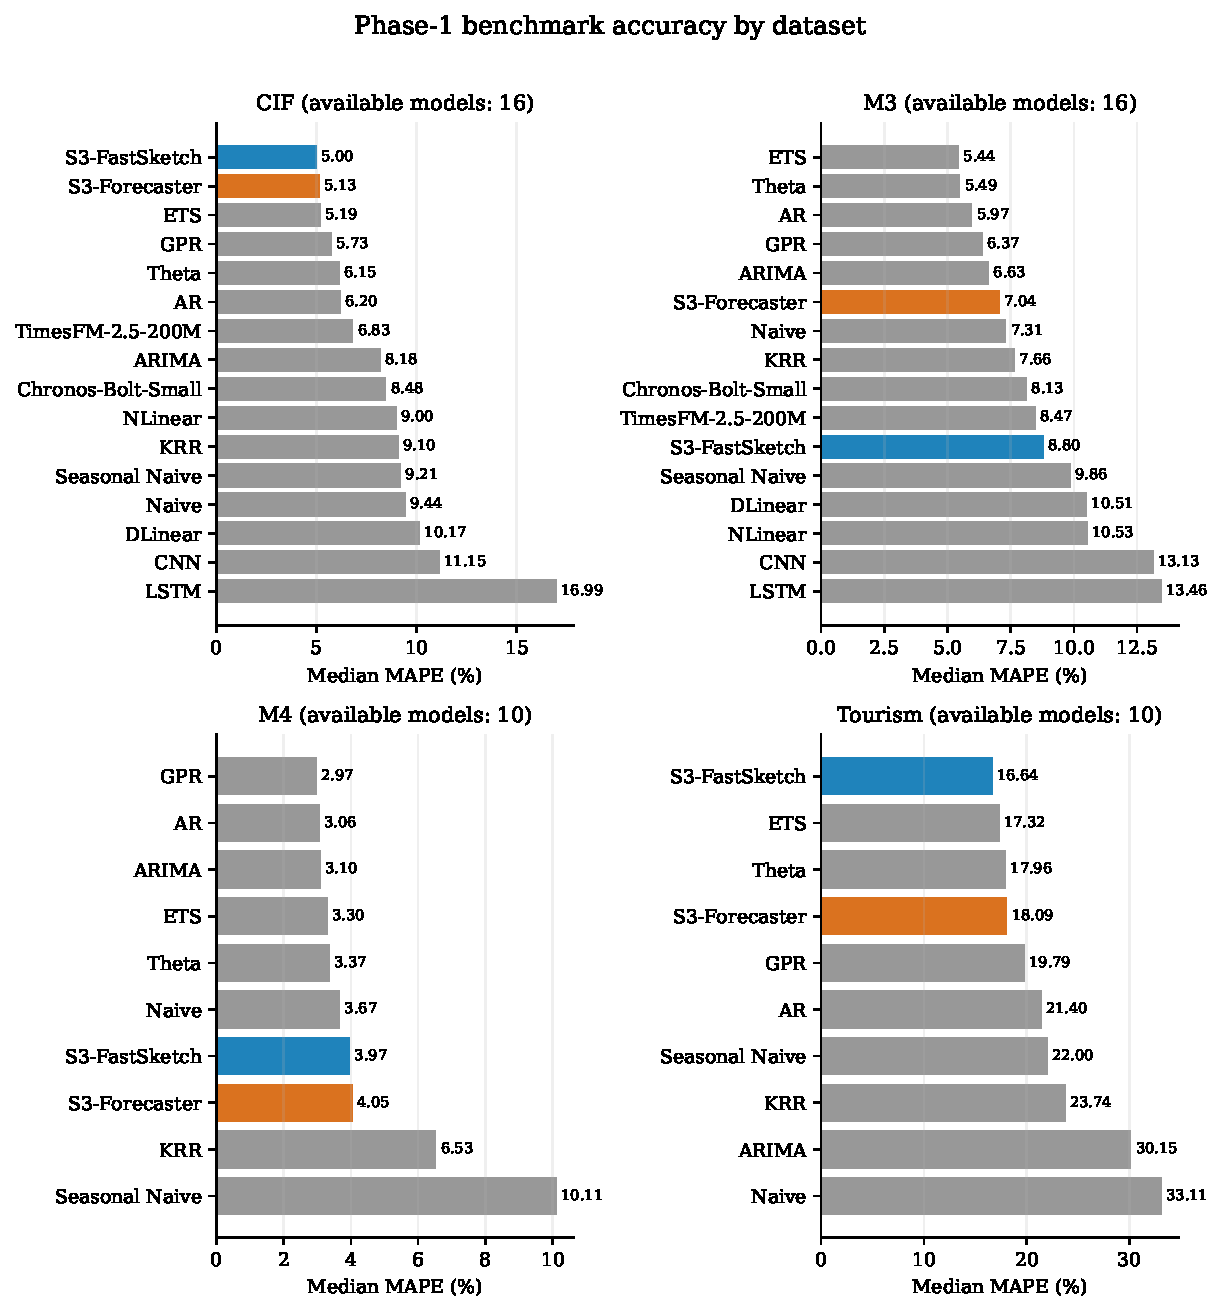
\includegraphics[width=0.93\textwidth]{figures/benchmark_mape_phase1.pdf}
    \caption{Median MAPE for the completed phase-1 benchmark runs. Blue and
    orange identify S3-FastSketch and S3-Forecaster, respectively. M4 and
    Tourism contain only the 10 currently completed models.}
    \label{fig:benchmark_mape_phase1}
\end{figure*}

On CIF, S3-FastSketch ranks first with a median MAPE of 4.996\%, followed by
S3-Forecaster at 5.133\%. The strongest completed non-S3 model is ETS at
5.189\%, so the improvement of S3-FastSketch over that reference is 3.7\% in
relative terms. The two S3 variants also precede the zero-shot foundation
models and the four trained neural baselines on this dataset. In particular,
DLinear, NLinear, CNN, and LSTM obtain median MAPEs of 10.166\%, 9.001\%,
11.155\%, and 16.993\%, respectively. This ordering is consistent with the
small-data motivation: increasing end-to-end trainable capacity does not
compensate automatically for limited series length.

Tourism provides a second favorable case. S3-FastSketch ranks first among the
10 completed models with a median MAPE of 16.643\%, compared with 17.319\% for
ETS and 17.964\% for Theta. This corresponds to a 3.9\% relative reduction with
respect to the best completed non-S3 comparator. S3-Forecaster is fourth at
18.091\%. The stronger result of the deterministic sketch variant suggests
that a fixed multiscale residual representation can be preferable to a richer
reservoir when the available signal is heterogeneous across many short series.
This interpretation remains provisional because the six neural and foundation
runs for Tourism are not yet present.

The results on M3 and M4 delimit the claim. On M3, ETS and Theta lead with
median MAPEs of 5.442\% and 5.489\%. S3-Forecaster ranks sixth at 7.038\%, while
S3-FastSketch ranks eleventh at 8.797\%. Nevertheless, S3-Forecaster remains
more accurate than Chronos-Bolt-Small, TimesFM-2.5-200M, DLinear, NLinear, CNN,
and LSTM in the completed M3 comparison. On M4, the two S3 variants rank seventh
and eighth with median MAPEs of 3.968\% and 4.046\%, whereas GPR leads at
2.972\%. Thus, the present evidence supports complementarity: the S3 family is
most useful when the frozen prior leaves a learnable residual structure, while
parsimonious statistical or kernel models remain stronger when that condition
is not satisfied.

Point accuracy and interval calibration do not move uniformly. S3-FastSketch
and S3-Forecaster obtain mean ECP values of 0.909 and 0.955 on CIF, but the
corresponding values are 0.837 and 0.933 on M3, 0.949 and 0.970 on M4, and 0.848
and 0.887 on Tourism. Relative to the nominal 0.90 target, the current intervals
therefore range from under-coverage to substantial over-coverage. The adaptive
conformal layer should consequently be presented as an online calibration
mechanism rather than as evidence of uniform finite-sample calibration across
all datasets. Shock-stratified interval diagnostics and the pending ICMD run
are required before making a stronger uncertainty claim.

\subsection{Data Efficiency Under Reduced Histories}
\label{subsec:data_efficiency_results}

Figure~\ref{fig:data_efficiency_phase1} and
Table~\ref{tab:data_efficiency_phase1} summarize the available reduced-history
runs. The trajectories are non-monotonic. For S3-FastSketch on CIF, median MAPE
falls from 5.983\% at 25\% history to 4.894\% at 75\%, and remains 4.996\% with
the full history. S3-Forecaster is stable between 50\% and 100\% history, with
median MAPE between 4.972\% and 5.133\%. On M3, S3-Forecaster reaches 6.110\%
at 25\% and 5.178\% at 50\%, but increases to approximately 7.0\% at 75\% and
100\%. A similar non-monotonic pattern occurs on M4: the 25\% values are
3.441\% for S3-FastSketch and 2.865\% for S3-Forecaster, while the corresponding
full-history values are 3.968\% and 4.046\%.

\begin{figure*}[t]
    \centering
    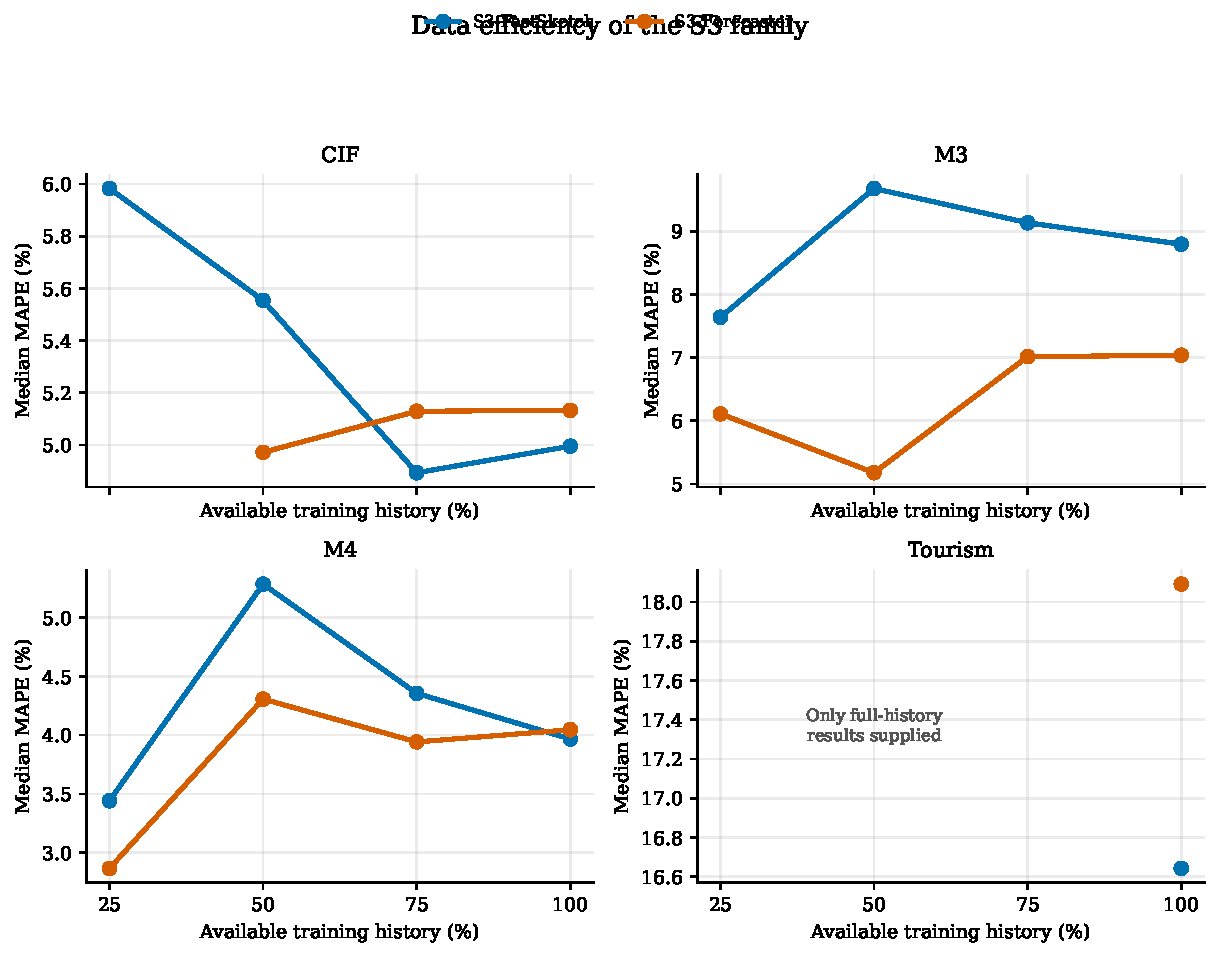
\includegraphics[width=0.88\textwidth]{figures/data_efficiency_phase1.pdf}
    \caption{Median MAPE of the S3 family as the available training history is
    reduced. Tourism currently contains only the full-history endpoints. The
    number of successfully evaluated series changes across some fractions.}
    \label{fig:data_efficiency_phase1}
\end{figure*}

\begin{table}[t]
\centering
\caption{Median MAPE (\%) as a function of the available training history.}
\label{tab:data_efficiency_phase1}
\footnotesize
\setlength{\tabcolsep}{4pt}
\begin{tabular}{llrrrr}
\toprule
Dataset & Model & 25\% ($n$) & 50\% ($n$) & 75\% ($n$) & 100\% ($n$) \\
\midrule
CIF & S3-FastSketch & 5.98 (47) & 5.55 (61) & 4.89 (65) & 5.00 (65) \\
CIF & S3-Forecaster & -- & 4.97 (53) & 5.13 (61) & 5.13 (65) \\
M3 & S3-FastSketch & 7.64 (149) & 9.68 (199) & 9.14 (199) & 8.80 (199) \\
M3 & S3-Forecaster & 6.11 (143) & 5.18 (155) & 7.02 (199) & 7.04 (199) \\
M4 & S3-FastSketch & 3.44 (153) & 5.29 (199) & 4.36 (199) & 3.97 (199) \\
M4 & S3-Forecaster & 2.87 (145) & 4.31 (199) & 3.94 (199) & 4.05 (199) \\
Tourism & S3-FastSketch & -- & -- & -- & 16.64 (199) \\
Tourism & S3-Forecaster & -- & -- & -- & 18.09 (199) \\
\bottomrule
\end{tabular}
\begin{minipage}{0.96\linewidth}
\footnotesize\emph{Note:} Each cell reports median MAPE followed by the number of successfully evaluated series in parentheses. Cohort size changes across fractions and, in some cases, across models; the trajectories are therefore descriptive rather than fixed-cohort learning curves. ``--'' denotes an unavailable run.
\end{minipage}
\end{table}


These values show that both architectures can remain operational with sharply
reduced histories, but they do not yet establish a monotonic learning curve.
The number of successfully evaluated series changes across fractions: for
example, the CIF S3-FastSketch cohort increases from 47 series at 25\% history
to 65 at full history, while the M4 S3-Forecaster cohort increases from 145 to
199. The current curves therefore combine a history-length effect with a cohort
composition effect. They should be interpreted as phase-1 feasibility evidence,
not as a causal estimate of the value of additional observations. The final
analysis should rerun every fraction on the intersection of series that is
valid for all models and fractions, and should report paired uncertainty for
the resulting changes.

The non-monotonic behavior is nevertheless scientifically informative. More
history is not automatically more useful under non-stationarity: older regimes
may dilute the local residual structure relevant to the test block, while
shorter histories may reduce model variance. This mechanism is compatible with
the design of S3, but it cannot be distinguished from cohort selection using
the aggregated export alone. No such causal attribution is made here.

\subsection{Shock Versus Non-Shock Behaviour}
\label{subsec:shock_results}

All 52 completed model--dataset combinations contain both shock and non-shock
summaries. Figure~\ref{fig:shock_penalty_phase1} reports the ratio between shock
and non-shock median MAPE, while Table~\ref{tab:shock_phase1} gives the absolute
values for the S3 family. A ratio above one indicates that accuracy deteriorates
on the observations classified as shocks.

\begin{figure*}[t]
    \centering
    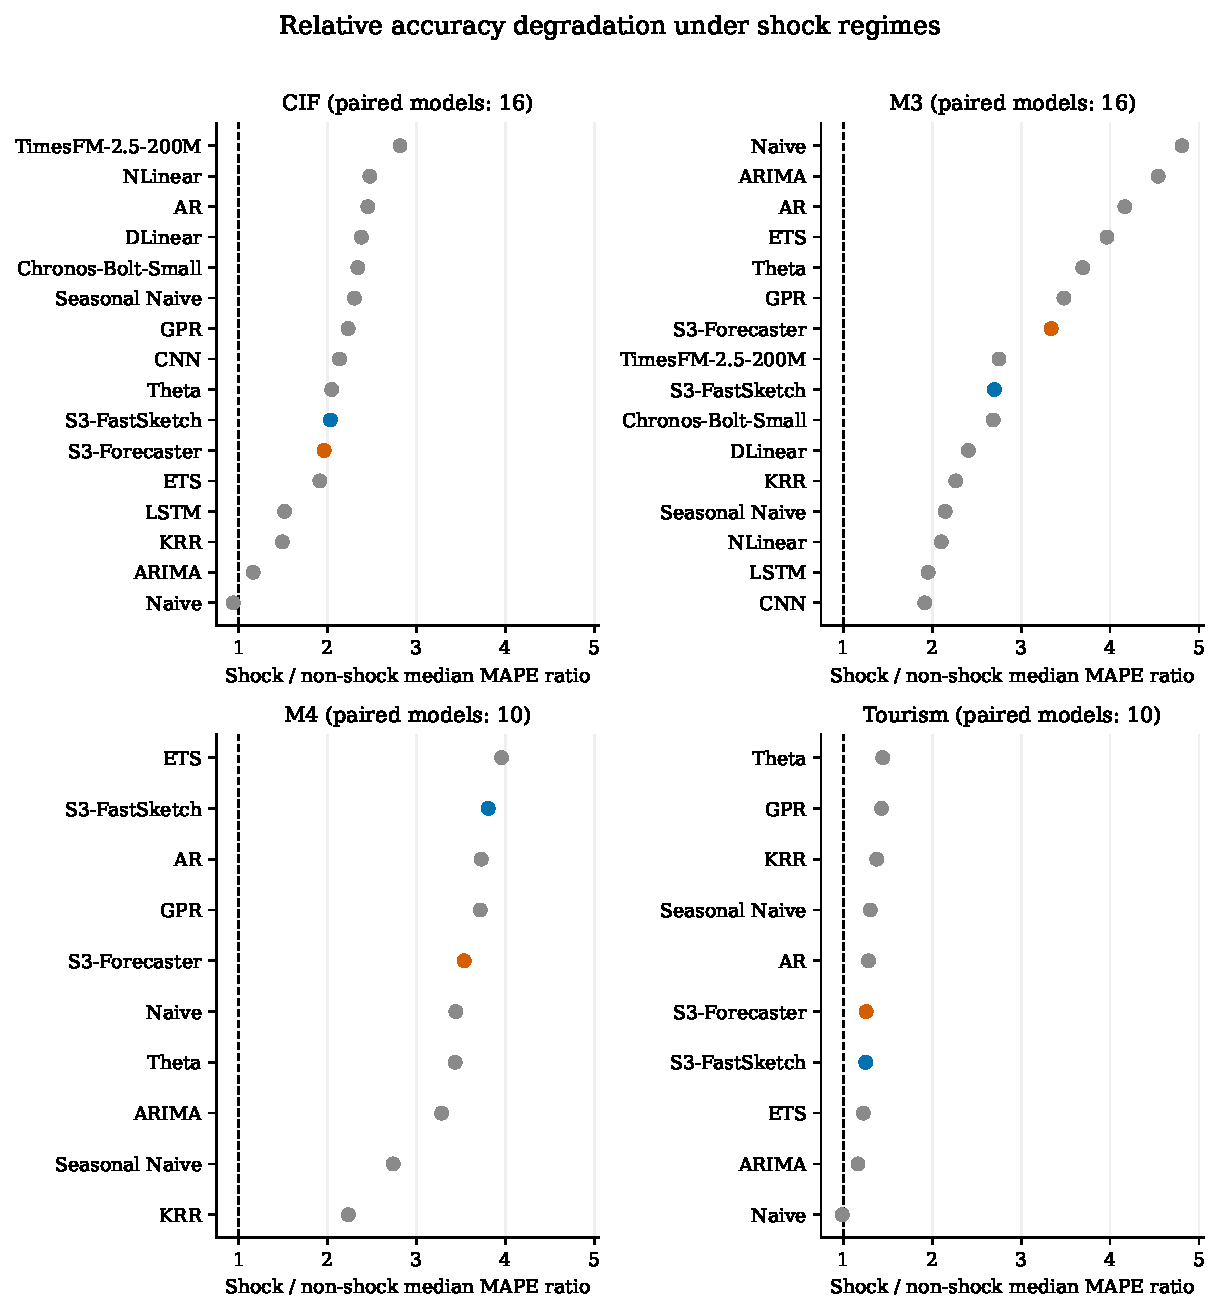
\includegraphics[width=0.91\textwidth]{figures/shock_penalty_phase1.pdf}
    \caption{Ratio of shock to non-shock median MAPE for each completed model.
    The dashed line denotes equal error in both regimes. Ratios must be read
    jointly with absolute error because a low ratio can result from poor
    non-shock performance.}
    \label{fig:shock_penalty_phase1}
\end{figure*}

\begin{table}[t]
\centering
\caption{Shock versus non-shock median MAPE for the S3 family.}
\label{tab:shock_phase1}
\footnotesize
\setlength{\tabcolsep}{4pt}
\begin{tabular}{llrrr}
\toprule
Dataset & Model & Non-shock (\%, $n$) & Shock (\%, $n$) & Ratio \\
\midrule
CIF & S3-FastSketch & 3.82 (40) & 7.77 (25) & 2.03 \\
CIF & S3-Forecaster & 4.05 (40) & 7.94 (25) & 1.96 \\
M3 & S3-FastSketch & 4.85 (88) & 13.08 (111) & 2.70 \\
M3 & S3-Forecaster & 2.95 (88) & 9.85 (111) & 3.34 \\
M4 & S3-FastSketch & 1.73 (83) & 6.59 (116) & 3.81 \\
M4 & S3-Forecaster & 1.82 (83) & 6.46 (116) & 3.54 \\
Tourism & S3-FastSketch & 14.92 (31) & 18.67 (168) & 1.25 \\
Tourism & S3-Forecaster & 14.90 (31) & 18.72 (168) & 1.26 \\
\bottomrule
\end{tabular}
\begin{minipage}{0.96\linewidth}
\footnotesize\emph{Note:} The ratio is shock MAPE divided by non-shock MAPE. Values above one indicate degradation during shock observations.
\end{minipage}
\end{table}


The regime split exposes a consistent challenge: most models deteriorate under
shocks, but the magnitude depends strongly on the dataset. On CIF, shock MAPE
is 7.771\% for S3-FastSketch and 7.940\% for S3-Forecaster, approximately twice
their non-shock errors of 3.821\% and 4.045\%. These absolute shock errors are
close to ETS at 7.500\%, while remaining below the shock errors of the neural
and foundation baselines. On Tourism, both S3 variants show a smaller relative
penalty: their shock/non-shock ratios are 1.25 and 1.26, with shock MAPEs of
18.666\% and 18.721\%. ETS is slightly better in absolute terms at 18.367\%,
whereas Theta reaches 19.446\%.

M3 and M4 are more difficult. On M3, S3-FastSketch rises from 4.849\% to
13.080\% and S3-Forecaster from 2.951\% to 9.848\%. Their ratios of 2.70 and
3.34 are lower than those of AR, ARIMA, ETS, and Naive, but S3 does not achieve
the lowest absolute shock error; Theta reaches 8.158\% and ETS 8.740\%. On M4,
the S3 shock errors are 6.589\% and 6.457\%, compared with 4.858\% for ETS and
5.002\% for AR. The shock-aware components therefore attenuate neither every
shock nor every dataset equally.

The two Naive ratios below one on CIF and Tourism should not be interpreted as
successful shock adaptation. In both cases the non-shock baseline error is
already high, so the ratio is reduced by a weak denominator reference. This is
why the absolute-regime table and the relative-penalty figure are reported
together. The current aggregate CSV also does not contain per-series paired
losses for statistical testing. The final manuscript should add confidence
intervals or paired resampling before claiming significant shock robustness.

\subsection{Ablation Evidence and Mechanistic Interpretation}
\label{subsec:ablation_results}

The ablation export contains 80 unique dataset--model--variant summaries and
uses the same number of evaluated series within each dataset--model block.
Figure~\ref{fig:ablation_phase1} reports the relative change in aggregated
median MAPE after removing one component. Positive values favor the full model;
negative values indicate that the ablated variant has lower median error.
Table~\ref{tab:ablation_extremes_phase1} lists the largest favorable and adverse
changes for each block.

\begin{figure*}[t]
    \centering
    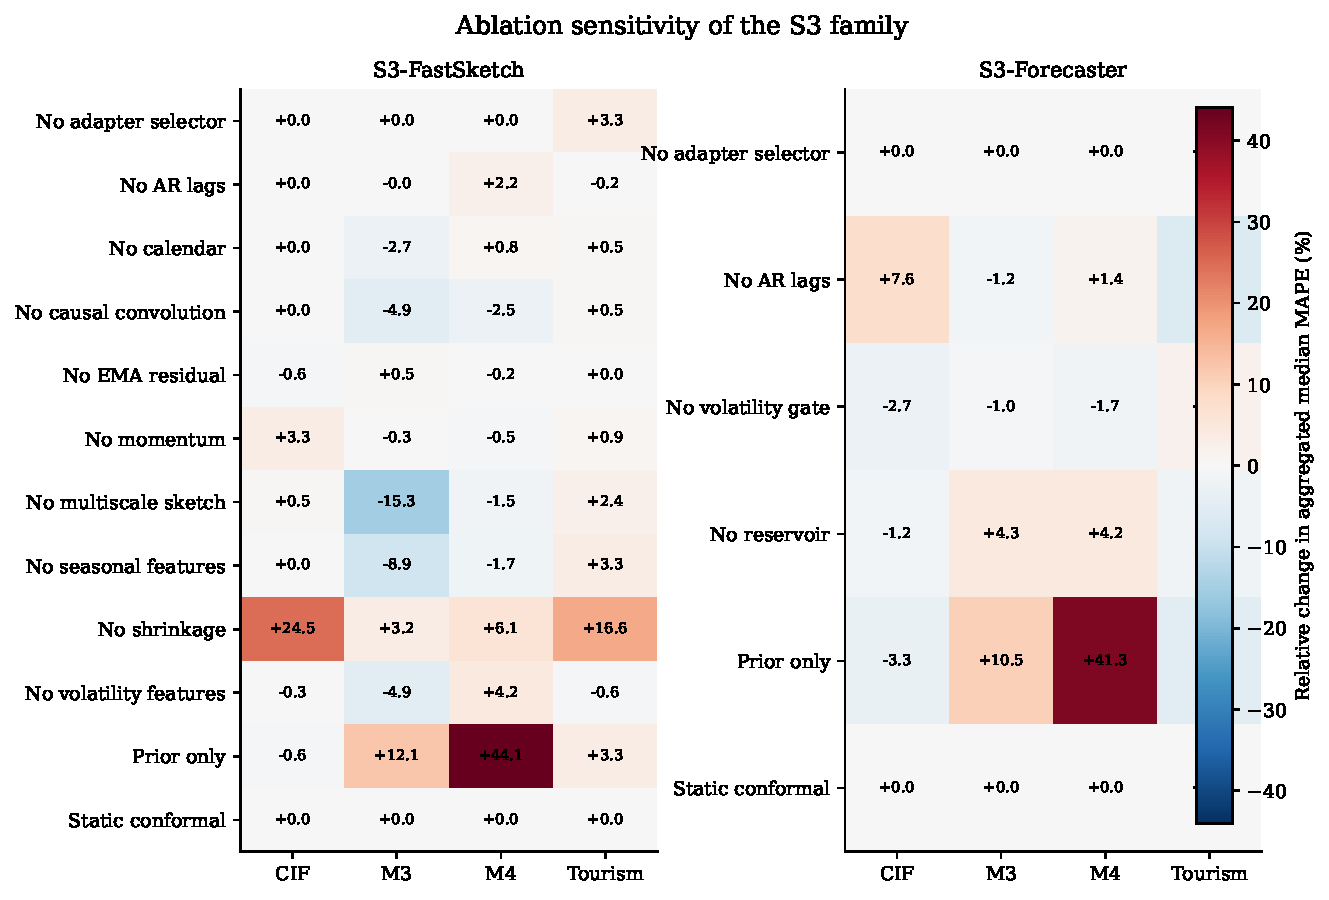
\includegraphics[width=0.92\textwidth]{figures/ablation_sensitivity_phase1.pdf}
    \caption{Relative change in aggregated median MAPE for the phase-1
    ablations. Positive values indicate degradation after removing the
    component. Blank cells denote variants that do not apply to an architecture.}
    \label{fig:ablation_phase1}
\end{figure*}

\begin{table*}[t]
\centering
\caption{Largest favorable and adverse paired median MAPE changes in the phase-1 ablation export.}
\label{tab:ablation_extremes_phase1}
\footnotesize
\setlength{\tabcolsep}{4pt}
\begin{tabular}{lllrlr}
\toprule
Dataset & Model & Most favorable removal & Change (\%) & Most adverse removal & Change (\%) \\
\midrule
CIF & S3-FastSketch & No EMA residual & -0.6 & No shrinkage & 24.5 \\
CIF & S3-Forecaster & Prior only & -3.3 & No AR lags & 7.6 \\
M3 & S3-FastSketch & No multiscale sketch & -15.3 & Prior only & 12.1 \\
M3 & S3-Forecaster & No AR lags & -1.2 & Prior only & 10.5 \\
M4 & S3-FastSketch & No causal convolution & -2.5 & Prior only & 44.1 \\
M4 & S3-Forecaster & No volatility gate & -1.7 & Prior only & 41.3 \\
Tourism & S3-FastSketch & No volatility features & -0.6 & No shrinkage & 16.6 \\
Tourism & S3-Forecaster & No AR lags & -6.1 & No volatility gate & 1.8 \\
\bottomrule
\end{tabular}
\begin{minipage}{0.98\textwidth}
\footnotesize\emph{Note:} Changes compare each variant's aggregated median MAPE with the corresponding full-model median. Negative values favor the ablated variant; positive values favor the full model. This descriptive summary does not establish statistical significance.
\end{minipage}
\end{table*}


Two mechanisms receive direct support. First, removing shrinkage from
S3-FastSketch increases median MAPE by 24.5\% on CIF and 16.6\% on Tourism.
This is consistent with shrinkage acting as a variance-control mechanism rather
than as a cosmetic regularizer. Second, replacing the adapted forecast with the
prior-only configuration is especially damaging on M4: median MAPE increases by
44.1\% for S3-FastSketch and 41.3\% for S3-Forecaster. Prior-only also increases
median MAPE by 12.1\% and 10.5\% on M3. These results show that residual
adaptation can add substantial value when the residual signal is exploitable.

The ablations also reveal components that are not universally beneficial.
Removing the multiscale sketch reduces the aggregated median MAPE of
S3-FastSketch by 15.3\% on M3, while removing autoregressive lags reduces the
S3-Forecaster median by 6.1\% on Tourism. Smaller favorable removals occur in
several other blocks. This is not evidence against the overall architecture;
it shows that a fixed feature inventory can inject variance when the
corresponding residual pattern is absent. The adapter selector and shrinkage
mechanisms are therefore central to the S3 argument: the architecture should be
judged by its ability to exploit useful residual structure while suppressing
unsupported corrections, not by an assumption that every feature group must
help on every dataset.

\subsection{Implications, Limitations, and Pending Evidence}
\label{subsec:discussion_implications}

The phase-1 results support a focused engineering claim. Low-capacity,
gradient-free residual adaptation can outperform statistical, trained neural,
and frozen foundation references on selected small-data collections, as shown
most clearly by the first-place S3-FastSketch results on CIF and Tourism. The
M3 and M4 outcomes prevent a stronger universal-superiority claim and instead
motivate an explicit model-selection perspective: S3 is most valuable when the
prior residual is stable enough to learn, and the prior-only or a classical
model remains preferable otherwise.

The neural results currently available for CIF and M3 also clarify the role of
LSTM and CNN in the final benchmark. Both models rank below the S3 family on
those datasets and require substantially more operational time than the
lightweight alternatives on M3. They remain useful as legacy trained-deep
controls, but the evidence does not justify making them the center of the main
comparison. Retaining them in the completed benchmark or supplementary material
is more defensible than removing all trained nonlinear sequence references.

Four limitations define the boundary of this draft. First, M4 and Tourism are
missing the six neural and foundation-model runs, so their ranks are
conditional. Second, the reduced-history cohorts are not fixed, preventing a
clean causal data-efficiency claim. Third, the shock and ablation exports are
aggregated summaries and do not support paired significance tests. Fourth, the
final ICMD and multi-prior robustness results are not included in the supplied
files. These gaps do not invalidate the present observations, but they must be
closed before submission. The final analysis should preserve the same
chronological protocol, freeze the evaluated cohort across data fractions,
report paired uncertainty, and update this section without extrapolating from
missing cells.

\FloatBarrier
